\documentclass[12pt, twoside]{article}
% \documentclass[12pt, twoside]{article}
\usepackage[letterpaper, margin=1in, headsep=0.2in]{geometry}
\setlength{\headheight}{0.6in}
%\usepackage[english]{babel}
\usepackage[utf8]{inputenc}
\usepackage{microtype}
\usepackage{amsmath}
\usepackage{amssymb}
%\usepackage{amsfonts}
\usepackage[nomessages]{fp} %\FPeval{\var-name}{2*sin(pi/6)}
\usepackage{siunitx} %units in math. eg 20\milli\meter
\usepackage{yhmath} % for arcs, overparenth command
\usepackage{tikz} %graphics
\usetikzlibrary{quotes, angles, arrows, arrows.meta}
\usepackage{graphicx} %consider setting \graphicspath{{images/}}
\usepackage{parskip} %no paragraph indent
\usepackage{enumitem}
\usepackage{multicol}
\usepackage{venndiagram}

\usepackage{fancyhdr}
\pagestyle{fancy}
\fancyhf{}
\renewcommand{\headrulewidth}{0pt} % disable the underline of the header
\raggedbottom
\hfuzz=2mm %suppresses overfull box warnings

\usepackage{hyperref}
\usepackage{float}

\fancyhead[LE]{\thepage}
\fancyhead[RO]{\thepage \\ First and last name: \hspace{2.5cm} \,\\ Section: \hspace{2.5cm} \,}
\fancyhead[LO]{BECA/Huson/Geometry: Construction \\* 10 October 2024}

\begin{document}
\subsubsection*{1.23 Midterm Exam: Constructions \& transformations}
\begin{enumerate}[itemsep=0.5cm]
\item Construct an equilateral triangle with one side $\overline{AB}$.  
  \vspace{5cm}
  \begin{center}
  \begin{tikzpicture}
    \draw [-, thick] (0,0)--(5,1);
    \draw [fill] (0,0) circle [radius=0.05] node[below]{$A$};
    \draw [fill] (5,1) circle [radius=0.05] node[below]{$B$};
  \end{tikzpicture}
  \end{center}

\item Construct an angle bisector of the given angle.
  \vspace{3cm}
  \begin{center}
  \begin{tikzpicture}
    \draw [<->, thick] (-7,2)--(0,0)--(0.5,7);
    %\draw [fill] (0,0) circle [radius=0.05] node[below]{$A$};
  \end{tikzpicture}
  \end{center} \vspace{1cm}

\newpage
\item Construct a perpendicular bisector of $\overline{PQ}$.  
  \vspace{4cm}
  \begin{center}
  \begin{tikzpicture}
    \draw [-, thick] (0,0)--(5,-2);
    \draw [fill] (0,0) circle [radius=0.05] node[below]{$P$};
    \draw [fill] (5,-2) circle [radius=0.05] node[below]{$Q$};
  \end{tikzpicture}
  \end{center} 
  \vspace{3cm}

\item Construct a perpendicular to line $l$ through the point $P$.  
    \vspace{4cm}
    \begin{center}
    \begin{tikzpicture}
        \draw [<->, thick] (0,0)--(10,-5) node [below right]{$l$};
        \draw [fill] (4.5,0) circle [radius=0.05] node[below right]{$P$};
    \end{tikzpicture}
    \end{center}

\newpage
\subsubsection*{1.23 Midterm Exam: Transformations}
\item Translate $\triangle ABC$ left five and down three units. Label the image $\triangle A'B'C'$.
\begin{center}
    \begin{tikzpicture}[scale=0.7]
    \draw [help lines] (-8,-6) grid (8,6);
    \draw [thick, <->] (-8.4,0) -- (8.4,0) node [right] {$x$};
    \draw [thick, <->] (0,-6.4)--(0,6.4) node [above] {$y$};  
    \draw [thick]
      (3,4) node[above right] {$A$}--
      (3,-2) node[below] {$B$}--
      (6,3) node[below right] {$C$}--cycle;  
  \end{tikzpicture}
\end{center}

\item Reflect $\triangle DEF$ across the $x$-axis, labeling the image $\triangle D'E'F'$.
\begin{center}
    \begin{tikzpicture}[scale=.7]
    \draw [help lines] (-8,-6) grid (8,6);
    \draw [thick, <->] (-8.4,0) -- (8.4,0) node [right] {$x$};
    \draw [thick, <->] (0,-6.4)--(0,6.4) node [above] {$y$};  
    \draw [thick]
      (2,1) node[above left] {$D$}--
      (7,4) node[above right] {$E$}--
      (7,1) node[below right] {$F$}--cycle;  
  \end{tikzpicture}
\end{center}

\newpage
\item Rotate the triangle $90^\circ$ clockwise around the origin, $\triangle ABC \rightarrow \triangle A'B'C'$. Complete the table of the coordinates and plot and label the image on the grid. \vspace{0.5cm}
\begin{multicols}{2}
  $A(0,0) \rightarrow$ \\[0.7cm]
  $B(2,4) \rightarrow$ \\[0.7cm]
  $C(2,0) \rightarrow$ \\[0.7cm]
    \begin{tikzpicture}[scale=.70]
    \draw [help lines] (-5,-5) grid (5,5);
    \draw [thick, <->] (-5.4,0) -- (5.4,0) node [right] {$x$};
    \draw [thick, <->] (0,-5.4)--(0,5.4) node [above] {$y$};  
    \draw [thick]
      (0,0) node[below left] {$A$}--
      (2,4) node[above right] {$B$}--
      (2,0) node[above right] {$C$}--cycle;  
    \end{tikzpicture}
  \end{multicols}

\item Triangle $X'Y'Z'$ is the image of triangle $XYZ$ after a translation. Which triangle is larger, or are they the same size? Justify your answer. \vspace{3cm}

\item A reflection maps $P(-5,3)$ onto $P'(5,3)$. Is the reflection across the $x$-axis or the $y$-axis? \vspace{2cm}

\item Specify the translation that maps $Q(-1,2)\rightarrow Q'(6,-5)$. \vspace{1cm}
\newpage

\item Simplify the expression by combining like terms.
    \begin{multicols}{2}
        \begin{enumerate}[itemsep=0.5cm]
          \item $2x+4-x+11$
          \item $5y-4-7y+y$
          \item $14+5\pi-2\pi+4$
          \item $2a-7a+3\sqrt{5}+\sqrt{5}$
        \end{enumerate}
    \end{multicols}

\item Use the function $f(x) = 5x-10$ to answer the questions.
\begin{multicols}{2}
\begin{enumerate}[itemsep=1cm]
    \item What is $f(3)$?
    \item Find $f(-1)$
    \item What is $x$ when $f(x) = 10$?
\end{enumerate}
\end{multicols} \vspace{1cm}

\end{enumerate}
\end{document}